\documentclass[a4paper,10pt]{article}

\usepackage[english]{babel}
\usepackage{amssymb}
\usepackage{fancyhdr}
\usepackage{graphicx}
\usepackage[ocgcolorlinks]{hyperref}
\usepackage{todonotes}
\usepackage{caption}
\usepackage{subcaption}
\usepackage{epstopdf}

\pagestyle{fancy}
\fancyhead{}
\fancyfoot{}
\fancyhead[RE,LO]{de Kok \& Methenitis}
\fancyhead[RO,LE]{Week 5 \& 6}
\fancyfoot[RE]{\thepage$\quad \square$}
\fancyfoot[LO]{$\square \quad$\thepage}

\title{Report for Week 5 \& 6\\\normalsize Create your own ``Google Similar Images'' system}

\author{Patrick de Kok (5640318) \and Georgios Methenitis (10407537)}

\begin{document}
\maketitle
\thispagestyle{empty}

\section{Implement $k$-NN classifier}
As asked for, the most similar images to the four query images \texttt{goal/15.jpg}, \texttt{bicycle/37.jpg}, \texttt{beach/31.jpg} and \texttt{mountain/37.jpg} are drawn in the report.  The images can be found in Figure~\ref{f:knns}.

\begin{figure}
  \begin{subfigure}{.47\textwidth}
    \centering
    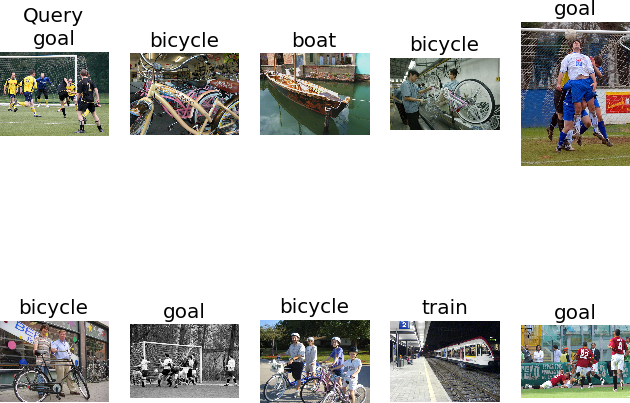
\includegraphics[width=1\textwidth]{knn_goal15}
    \caption{Query image \texttt{goal/15.jpg}.}
  \end{subfigure}
  \hspace*{\fill}
  \begin{subfigure}{.47\textwidth}
    \centering
    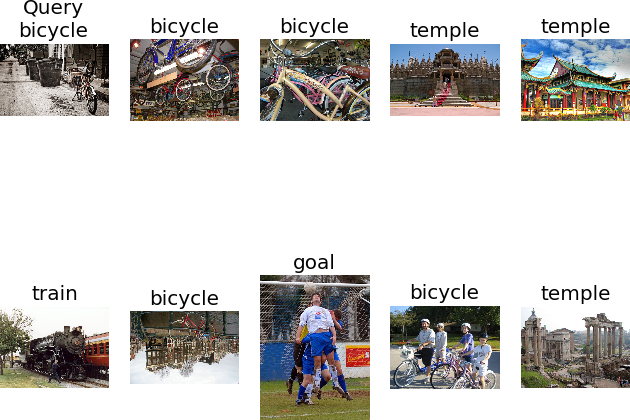
\includegraphics[width=1\textwidth]{knn_bicycle37}
    \caption{Query image \texttt{bicycle/37.jpg}.}
  \end{subfigure}

  \begin{subfigure}{.47\textwidth}
    \centering
    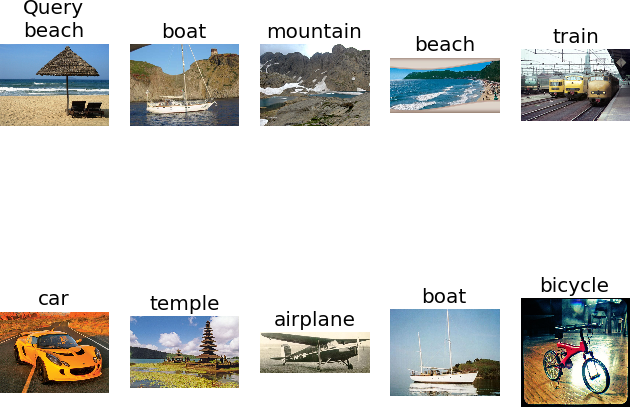
\includegraphics[width=1\textwidth]{knn_beach31}
    \caption{Query image \texttt{beach/31.jpg}.}
  \end{subfigure}
  \hspace*{\fill}
  \begin{subfigure}{.47\textwidth}
    \centering
    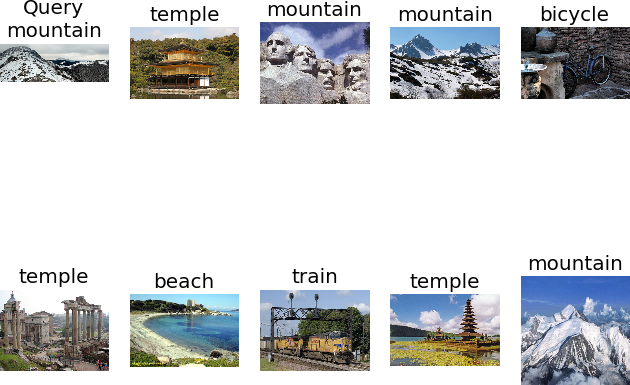
\includegraphics[width=1\textwidth]{knn_mountain37}
    \caption{Query image \texttt{mountain/37.jpg}.}
  \end{subfigure}
  \caption{Query images and their $k=9$ nearest neighbours with labels.}
  \label{f:knns}
\end{figure}

\section{Different $k$-NN strategy}
A possible alternative to this simple voting mechanism will be by weighing each vote based on its rank.  Each vote with rank $r$ will be assigned a weight \[ w_r = \frac{1}{1+r}. \]  Images with a higher rank should be considered as more important than lower ranked images.  The addition of 1 to the rank in the denominator lets the first vote have less relative significance to the second and third votes, such that $w_1 < w_2 + w_3$.

Another weighing mechanism would be based on the global label frequency.  Votes for each label would be weighed by: \[ w_\ell = \frac{1}{\#\ell} \] where $\#\ell$ represents the frequency of label $\ell$ occurring among the training images.  One might want to normalize these weights before they are used, such that \[\bar w_\ell = \frac{w_\ell}{\sum_{\ell \in L} w_\ell}. \] Here, $L$ is the set of all labels.  This ensures that \[\sum_{\ell \in L} w_\ell = 1.\] By weighing votes of very frequent labels less and very infrequent labels more, we tell the system that when a rare (or common) label is suspected to occur in the image this is very (or less) significant than expected.

With training sets of limited size, one is often interested in applying a smoothing method over these weights, such as Good-Turing smoothing.  This will even out the pure chance occurance of very frequent labels and very infrequent labels.  Because this dataset has equal frequencies for all labels, this method is not applicable, and only the first method is implemented.

The accuracy for the original $k$-NN implementation over the four queries is $0.5$, while the alternative implementation has an accuracy of $0.25$.  When inspecting the nearest neighbours of the four queries visually, it becomes clear that the histogram intersection distance is not appropriate for this domain.  The best label is most often not the first returned by $k$-NN.

\section{Implement mean class accuracy}
The accuracy evaluation measure has been implemented, and both $k$-NN label selection mechanisms are evaluated with $k=9$.  The accuracies of both methods per image class and the mean accuracy can be found in Table~\ref{t:classacc}.  Overall both methods have difficulties classifying images correctly.  

\begin{table}
  \centering
  \begin{tabular}{l|rr}
    Class & Original $k$-NN & Alternative $k$-NN \\
    \hline
    Airplane & 0.5 & 0.2 \\
    Beach & 0.1 & 0.1 \\
    Bicycle & 0.8 & 0.7 \\
    Boat & 0.2 & 0.3 \\
    Car & 0.4 & 0.2 \\
    Flower & 0.4 & 0.3 \\
    Goal & 0.1 & 0.2 \\
    Mountain & 0.3 & 0.2 \\
    Temple & 0.3 & 0.3 \\
    Train & 0.0 & 0.1 \\
    \hline
    \emph{Mean accuracy} & 0.31 & 0.26
  \end{tabular}
  \caption{Class accuracy per class and the mean accuracy over the complete test set with the original $k$-NN.}
  \label{t:classacc}
\end{table}

\section{Cross validation of $k$}
The mean class accuracy for each value of $k \in \left\{1, 3, 5, 7, 9, 15\right\}$ is reported in Table~\ref{t:crossacc}.  This has only been computed for the label selection mechanism as meant in the first question.  With $k=9$, you will get the highest mean accuracy.

\begin{table}
  \centering
  \begin{tabular}{l|rrrrrr}
    Label &  $k=1$ &  $k=3$ &  $k=5$ &  $k=7$ &  $k=9$ &  $k=15$ \\
    \hline
    Airplane  & 0.120  & 0.262  & 0.201  & 0.181  & 0.222  & 0.181 \\
       Beach  & 0.312  & 0.348  & 0.332  & 0.257  & 0.173  & 0.201 \\
     Bicycle  & 0.459  & 0.685  & 0.597  & 0.623  & 0.645  & 0.702 \\
        Boat  & 0.348  & 0.363  & 0.363  & 0.458  & 0.423  & 0.423 \\
         Car  & 0.261  & 0.244  & 0.283  & 0.350  & 0.311  & 0.333 \\
      Flower  & 0.486  & 0.399  & 0.418  & 0.381  & 0.401  & 0.374 \\
        Goal  & 0.156  & 0.062  & 0.130  & 0.124  & 0.084  & 0.068 \\
    Mountain  & 0.308  & 0.153  & 0.281  & 0.329  & 0.446  & 0.467 \\
      Temple  & 0.160  & 0.080  & 0.197  & 0.192  & 0.210  & 0.234 \\
       Train  & 0.097  & 0.013  & 0.013  & 0.013  & 0.000  & 0.000 \\
    \hline
  \emph{Mean} & 0.274  & 0.266  & 0.284  & 0.292  & 0.294  & 0.292 \\
  \end{tabular}
  \caption{Class accuracies and mean accuracy for different values of $k$ with threefold cross validation.  As can be concluded from the mean, the classifier performs best with $k=9$.}
  \label{t:crossacc}
\end{table}

\section{Evaluation of 4 possible classifiers}
In this part of the assignment we visualize the data obtained by the four different classifiers. Figure~\ref{fig:4classifiers} shows the resulted predicted labels and the true labels of the four classifiers, as well as the error margin of each one of the classifiers. We can see that the fourth classifier for $classifier = 3$, we obtain the minimum margin error, so we can say that this classifier is the support vector machines.

\begin{figure}[ht!]
    \centering
    \begin{subfigure}{.49\textwidth}
    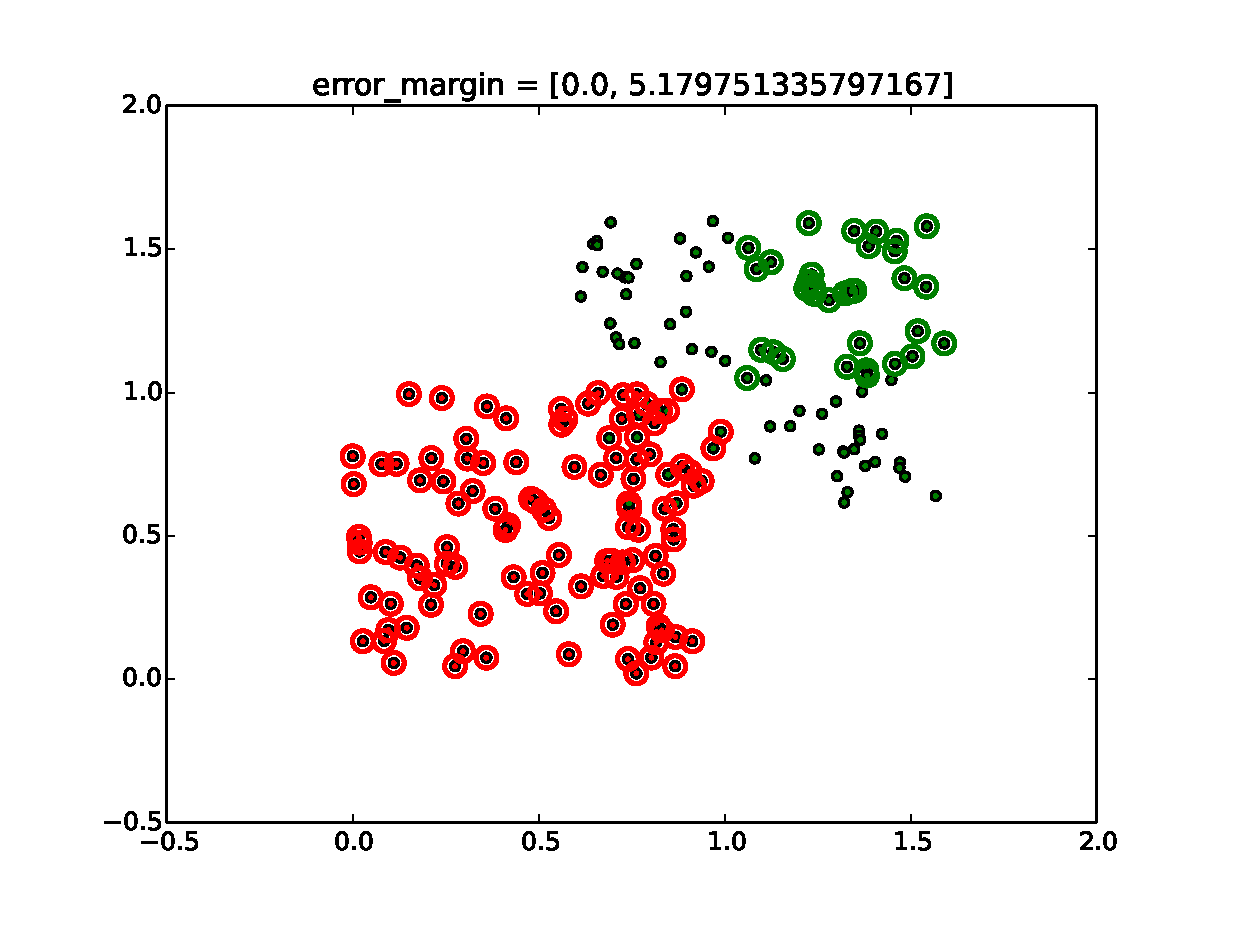
\includegraphics[width=1.00\textwidth]{svm1minError.eps}
    \caption{Classifier 1}
    \end{subfigure}
    \begin{subfigure}{.49\textwidth}
    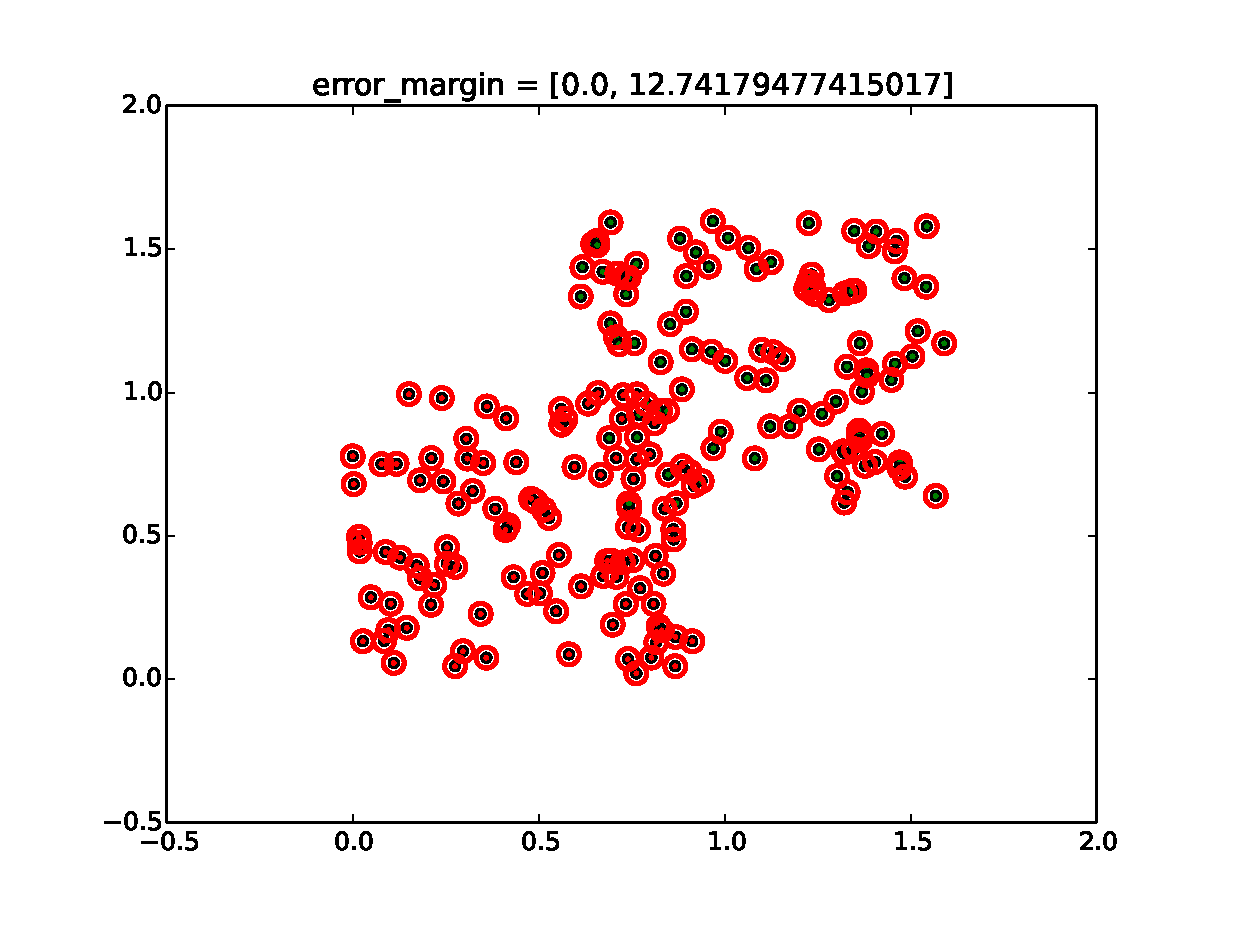
\includegraphics[width=1.00\textwidth]{svm2minError.eps}
    \caption{Classifier 2}
    \end{subfigure}
    \begin{subfigure}{.49\textwidth}
    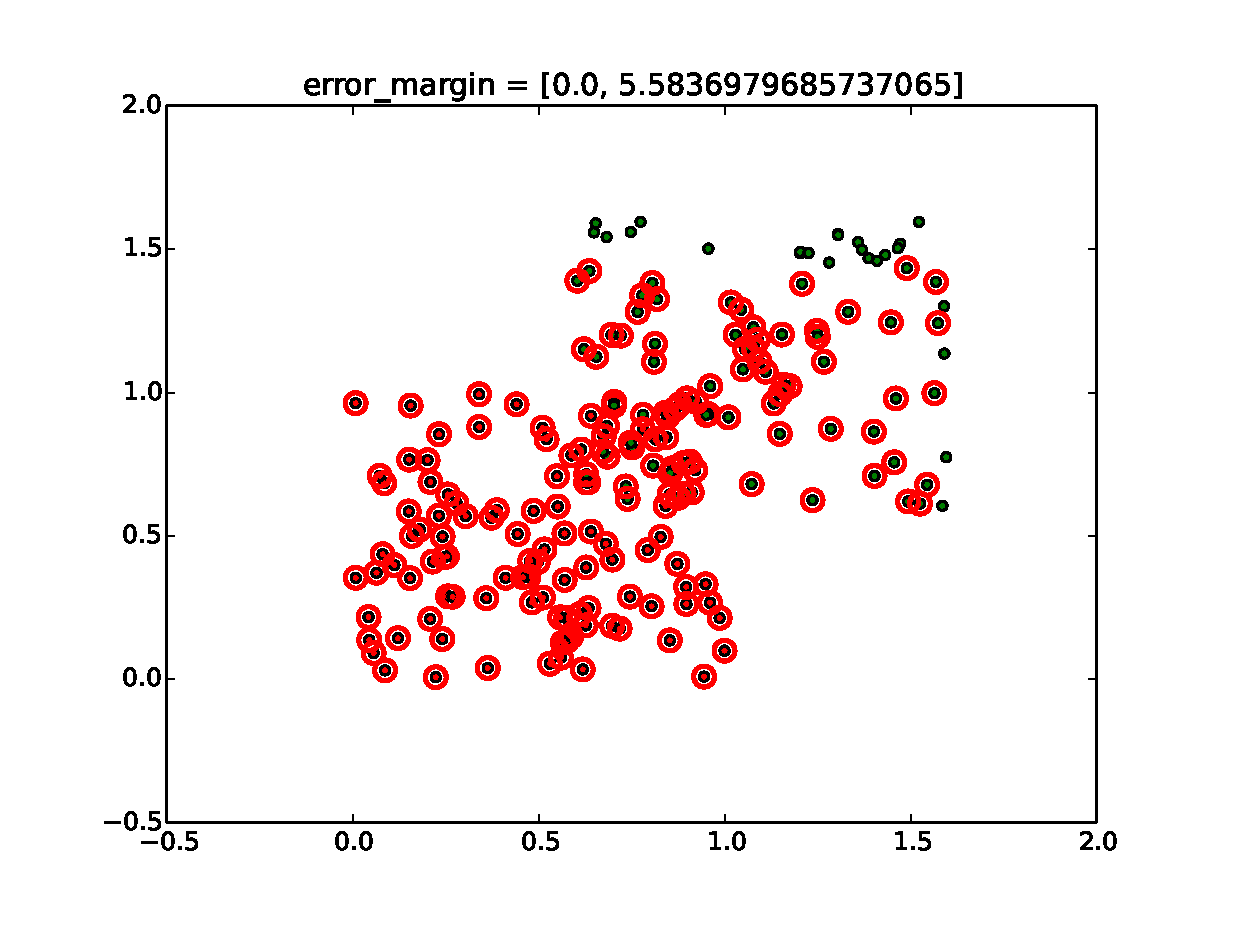
\includegraphics[width=1.00\textwidth]{svm3minError.eps}
    \caption{Classifier 3}
    \end{subfigure}
    \begin{subfigure}{.49\textwidth}
    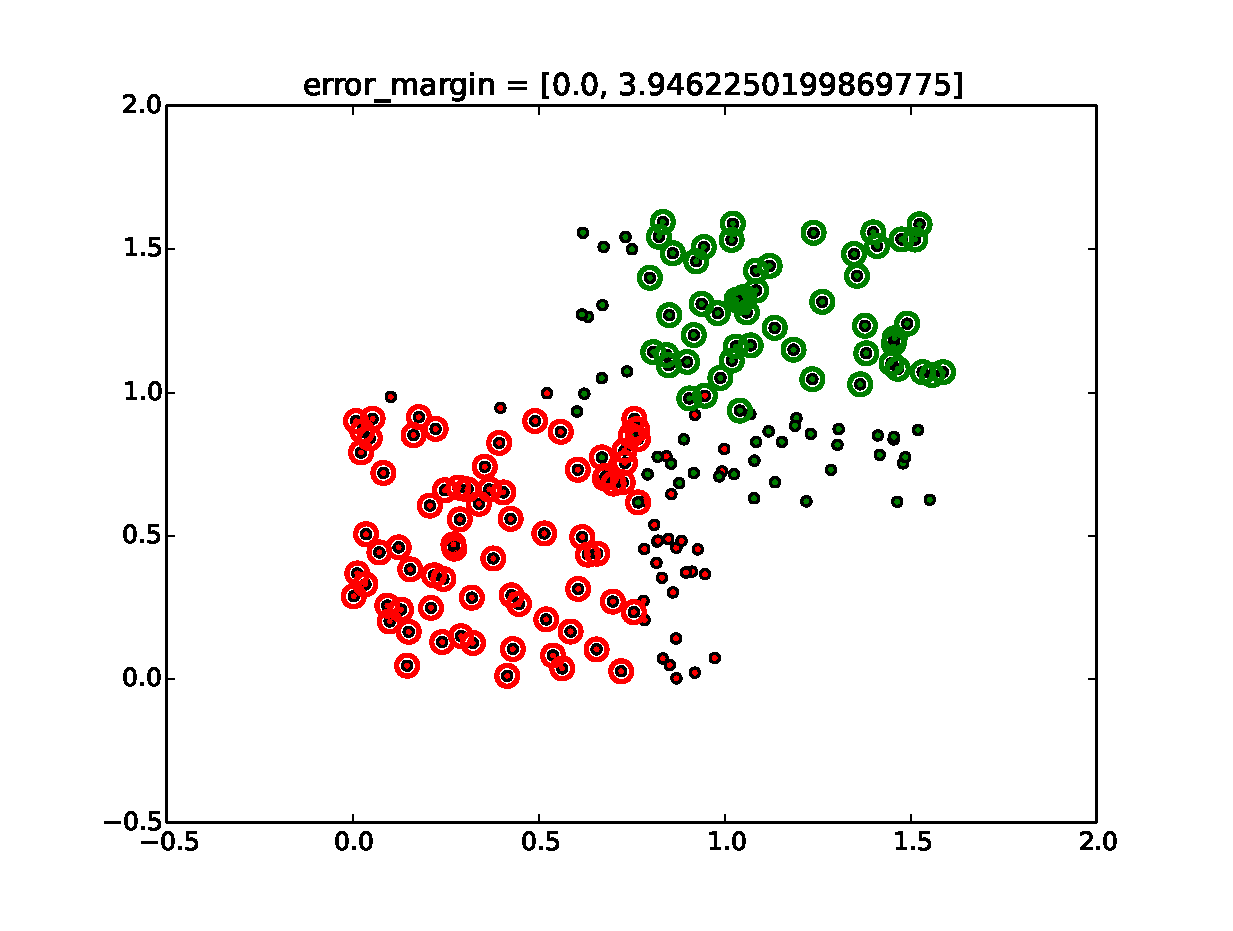
\includegraphics[width=1.00\textwidth]{svm4minError.eps}
    \caption{Classifier 4}
    \end{subfigure}
    \caption{Visualization of the four different classifiers.  The color of the center of a point indicates its true class.  The color of the outer circle indicates the predicted class by the classifier.  Error margins are reported above the image for both classes.}
    \label{fig:4classifiers}
\end{figure}

\section{Use scikit}
Now we apply the linear classifier from the \texttt{sklearn} package to train it on the provided data and the labels. Using a linear kernel, and $C = 1$ as it comes from default, the resulting predicted labels are shown in Figure~\ref{fig:linearClass}.
\begin{figure}[ht!]
    \centering
    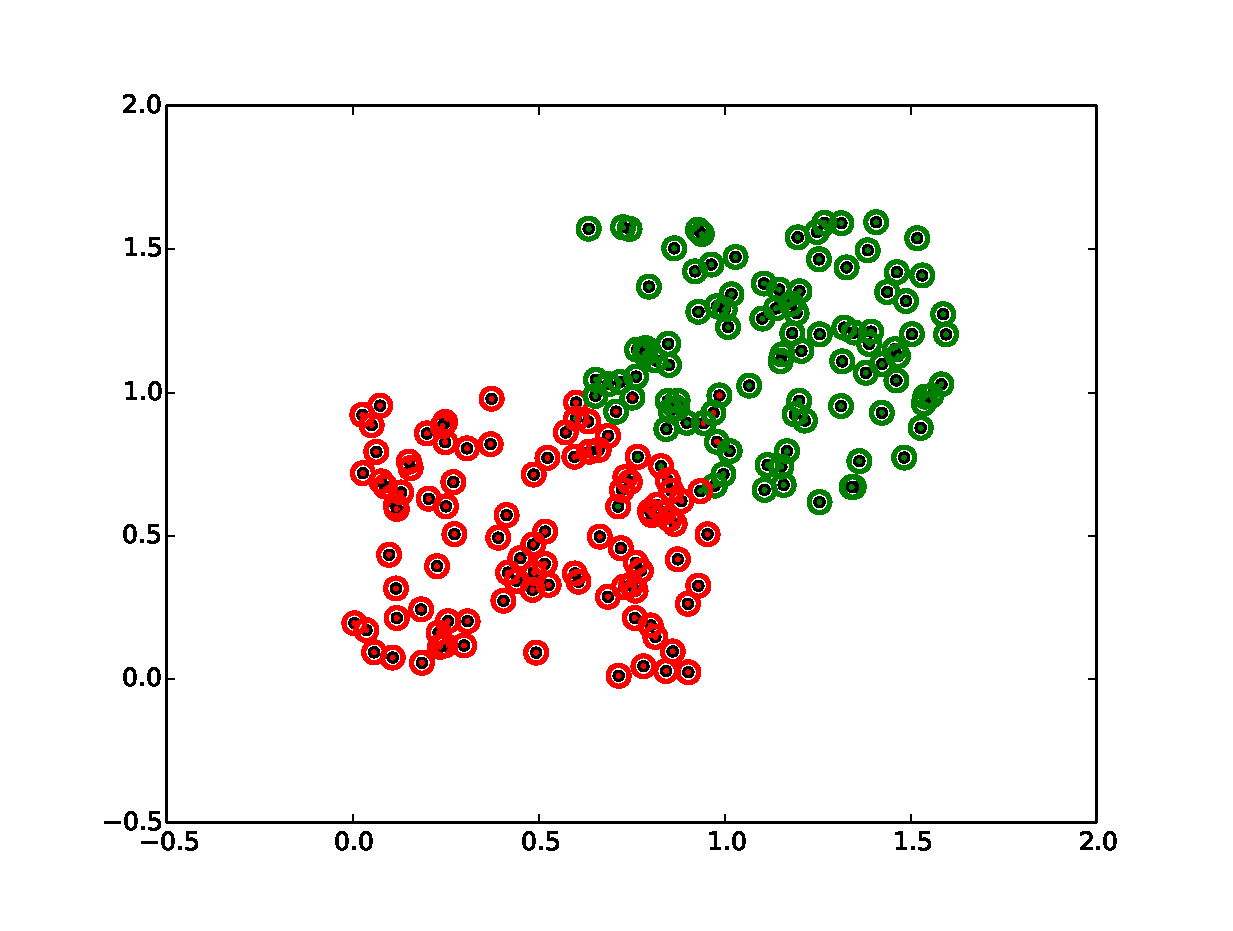
\includegraphics[width=1.00\textwidth]{svmFit.eps}
    \caption{Visualization of the predicted label of the model fitted by a linear SVM classifier.}
    \label{fig:linearClass}
\end{figure}

We can see that the predicted class for each data point is in most cases correct, with some faulty prediction only near the boundary between the two classes. This is happening because our classifier uses only one vector, and data from different classes are inside the area of the other class. We cannot overcome this problem with a linear classifier.  The data is not linearly separable; there is no straight line to separate both classes perfectly.
    
\section{Ring data -- linear SVM}
We run a linear SVM classifier on the ring data and we have visualized the predicted classes as well as the true class of each data point in Figure~\ref{fig:ringLinear}. The prediction accuracy of about $0.5$ is really bad as each predicted class contains only half of the correct class and half of the data of the wrong predicted class. We cannot predict the classes correctly as a linear vector classifier cannot distinguish over data that follow this patterns.  This is again because the data cannot be linearly separated. We tried also a non-linear classifier over these data points and the predicted classes were correct as non-linear classifiers can work with this type of data. 

The classification results can be seen in Figure~\ref{fig:ringLinear}.

\begin{figure}[ht!]
    \centering
    \begin{subfigure}{.49\textwidth}
    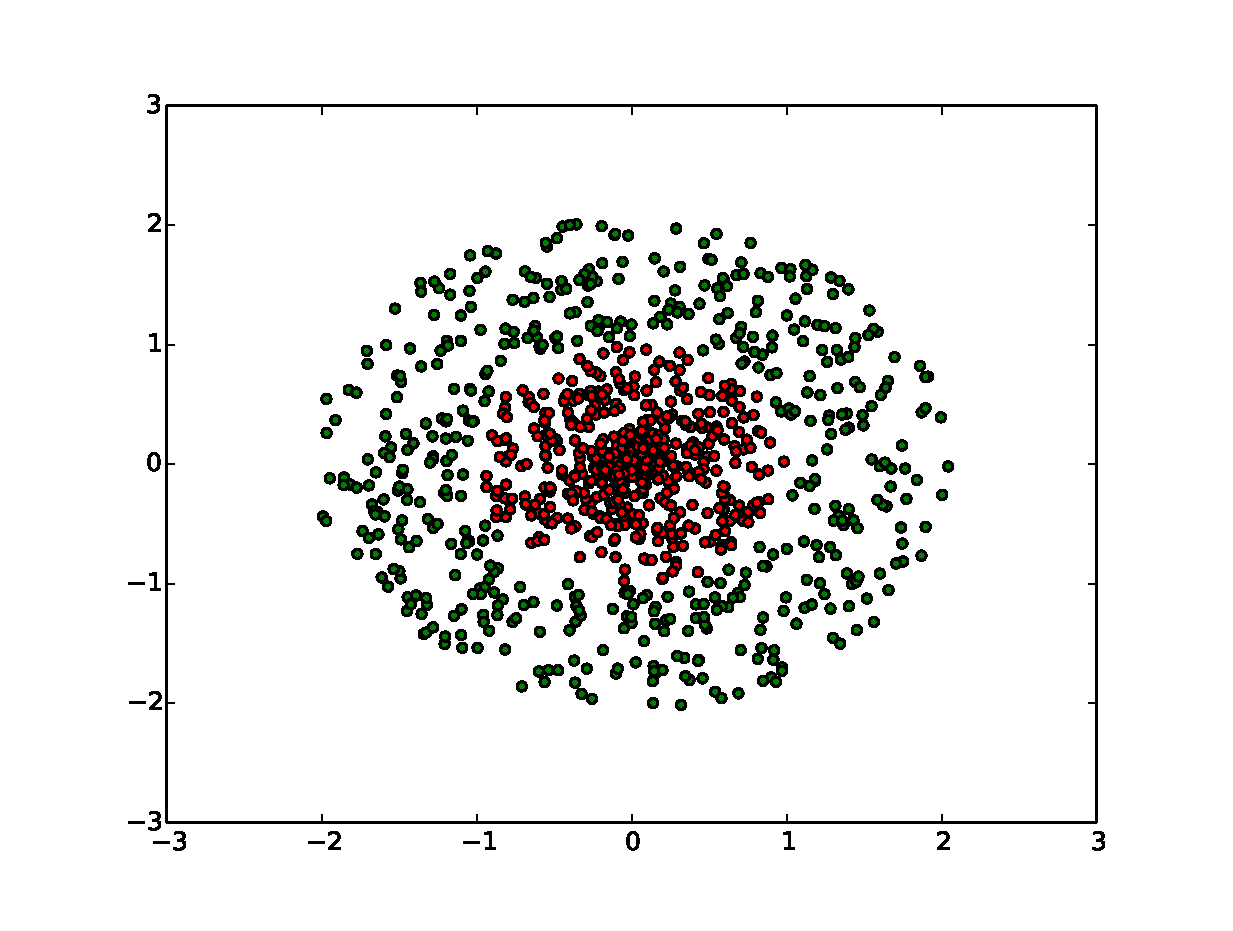
\includegraphics[width=1.00\textwidth]{ringData.eps}
    \caption{Ring data.}
    \end{subfigure}
    \begin{subfigure}{.49\textwidth}
    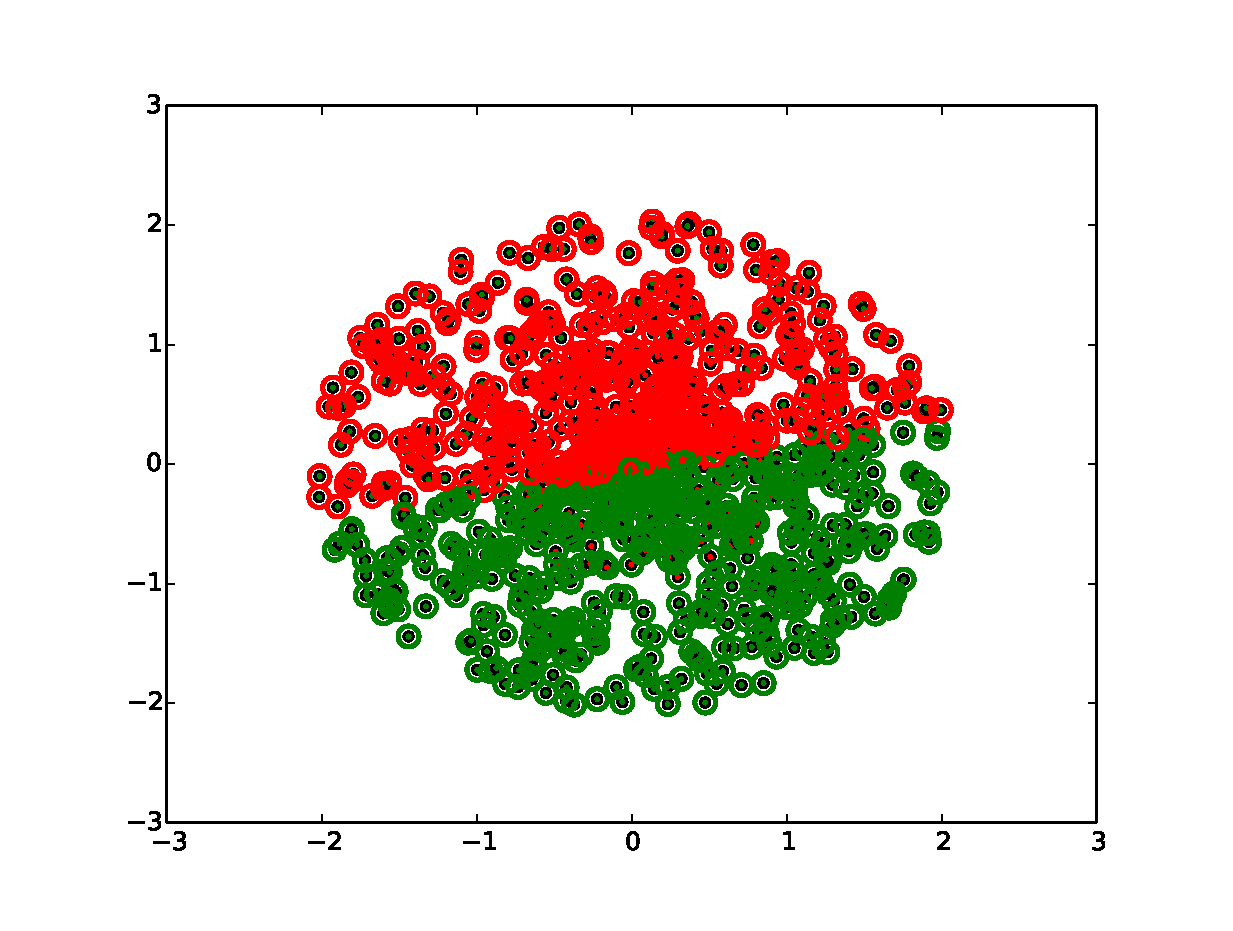
\includegraphics[width=1.00\textwidth]{ringLinearFit.eps}
    \caption{Predicted classes with a linear classifier.}
    \end{subfigure}
    \begin{subfigure}{.49\textwidth}
    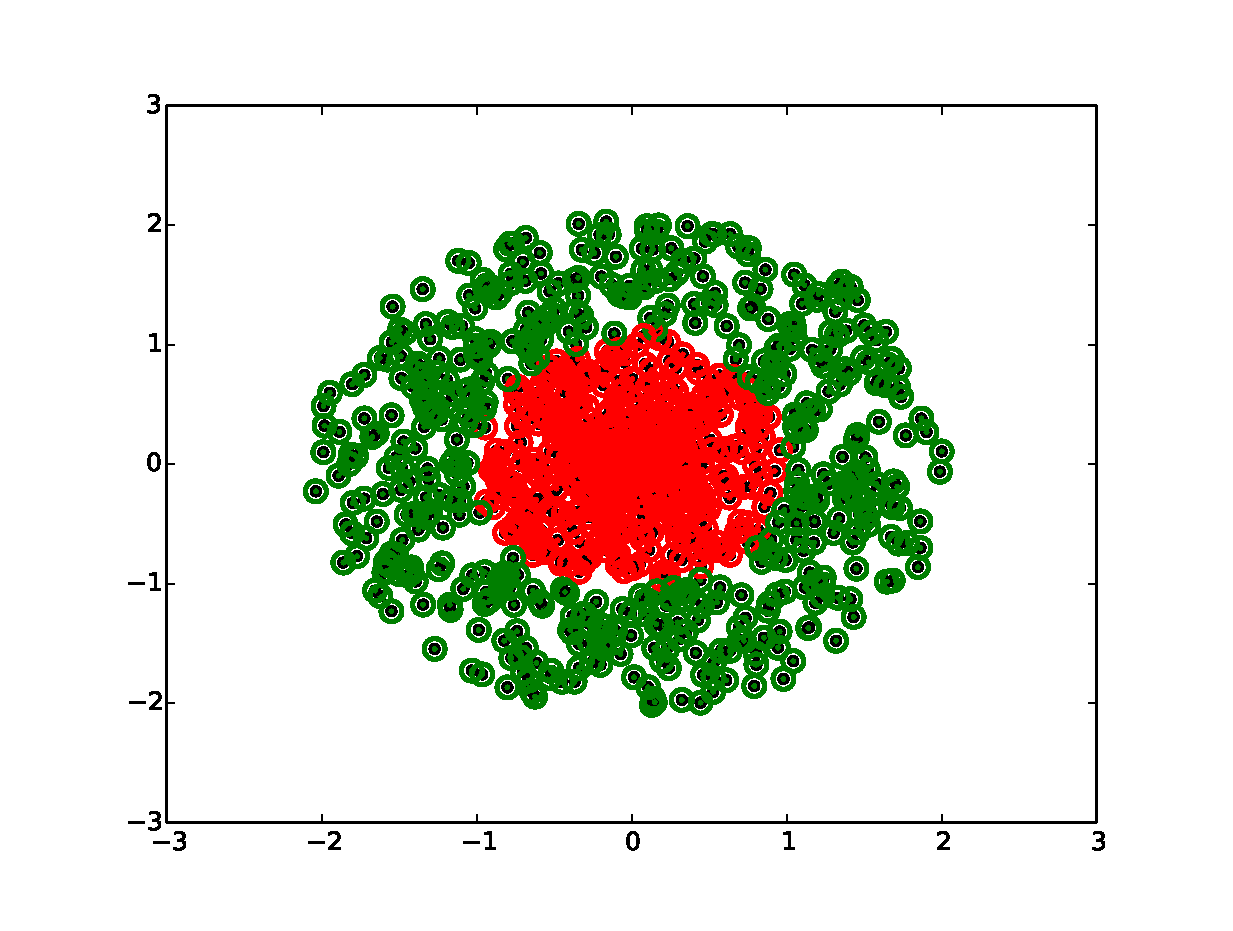
\includegraphics[width=1.00\textwidth]{ringNonLinearFit.eps}
    \caption{Predicted classes with a non-linear classifier.}
    \end{subfigure}
    \caption{Visualization of the predicted label of the ring data model fitted by a linear and a non-linear SVM classifier.  The same visualization technique has been used as described at Figure~\ref{fig:4classifiers}.}
    \label{fig:ringLinear}
\end{figure}


\section{Non-linear transformations}
The first approach to a non-linear transformation of the data is to represent points by their polar coordinates.  Each data point can be transformed as follows:
\begin{equation}
p(x,y) \rightarrow p'(\sqrt{x^2 + y^2}, \arctan(y,x))
\label{eq:2dpolar}
\end{equation}
In our case in which angle does not help us distinguish between the classes as all data points are equally distributed over all angles we could do the same without using the second term like:
\begin{equation}
p(x,y) \rightarrow p'(\sqrt{x^2 + y^2})
\end{equation}
Now we transformed the two-dimensional dataset to a one-dimensional space, make it feasible and easier than with Eq.~\ref{eq:2dpolar} to work with a linear classifier with one-dimensional data. As the only thing that we care about is the distance from the point $\left<0,0\right>$, we only use that piece of information. Another non-linear transformation that we could use in general, but would not be advisable in this case, is the following:
\begin{equation}
p(x,y) \rightarrow p'(x^2 - y^2, 2xy)
\end{equation}

\section{Transform to polar coordinates}
In this step we transformed all data into polar coordinates. Figure~\ref{fig:polarData} illustrates the resulted data points after the transformation.
\begin{figure}[ht!]
    \centering
    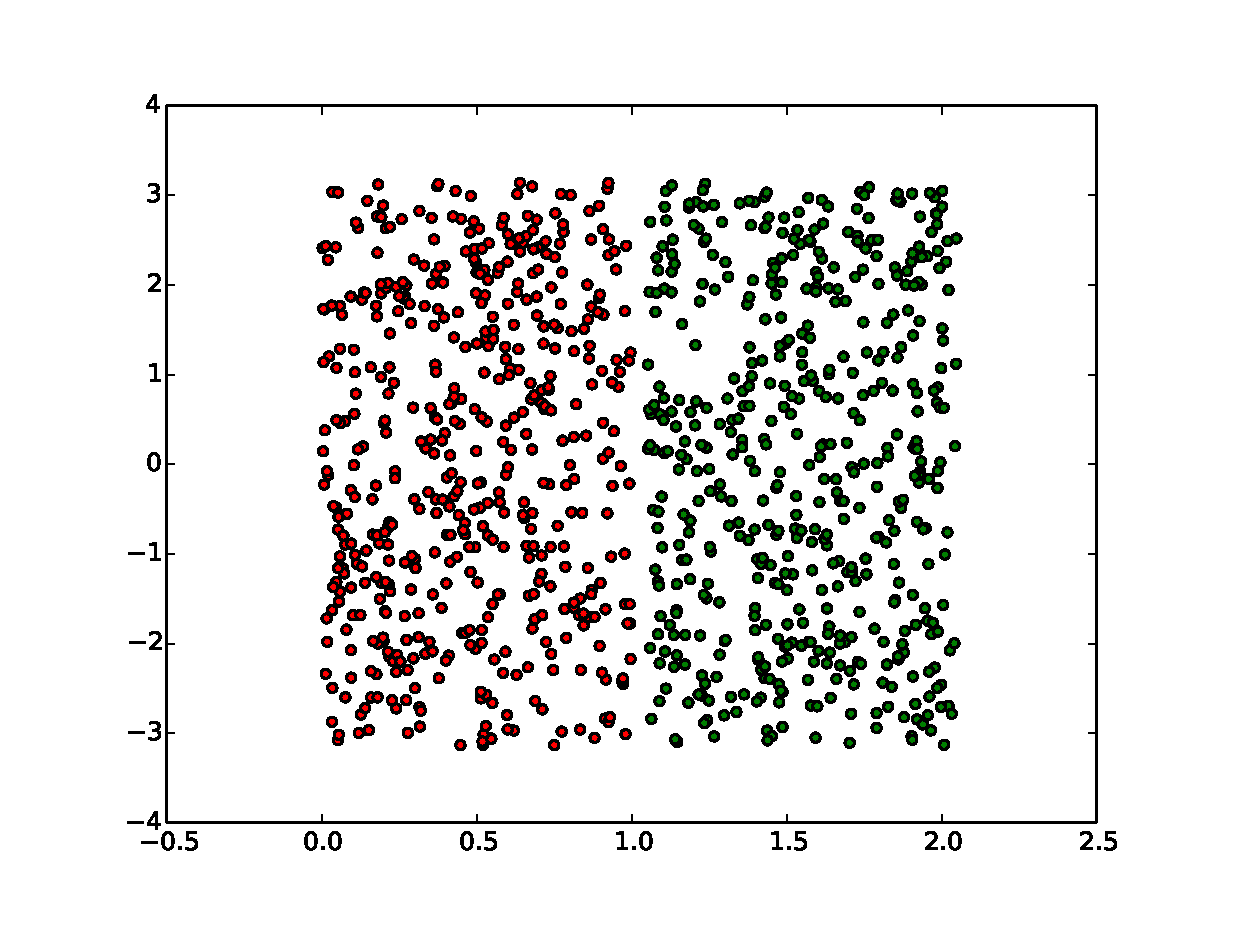
\includegraphics[width=0.70\textwidth]{polarData.eps}
    \caption{Ring data transformed into polar coordinates.}
    \label{fig:polarData}
\end{figure}

\section{Non-linear SVM}
Transforming the data into polar coordinates really improves the accuracy from $\sim 0.53$ to $\sim 1.00$, which we saw in Figure~\ref{fig:ringLinear}, and has better results than performing a non-linear classifier over the same data $\sim 0.99$. Figure~\ref{fig:linearSVMonPolar} shows the resulted predicted classes over the polar data representation and over the original data representation.
\begin{figure}[ht!]
    \centering
    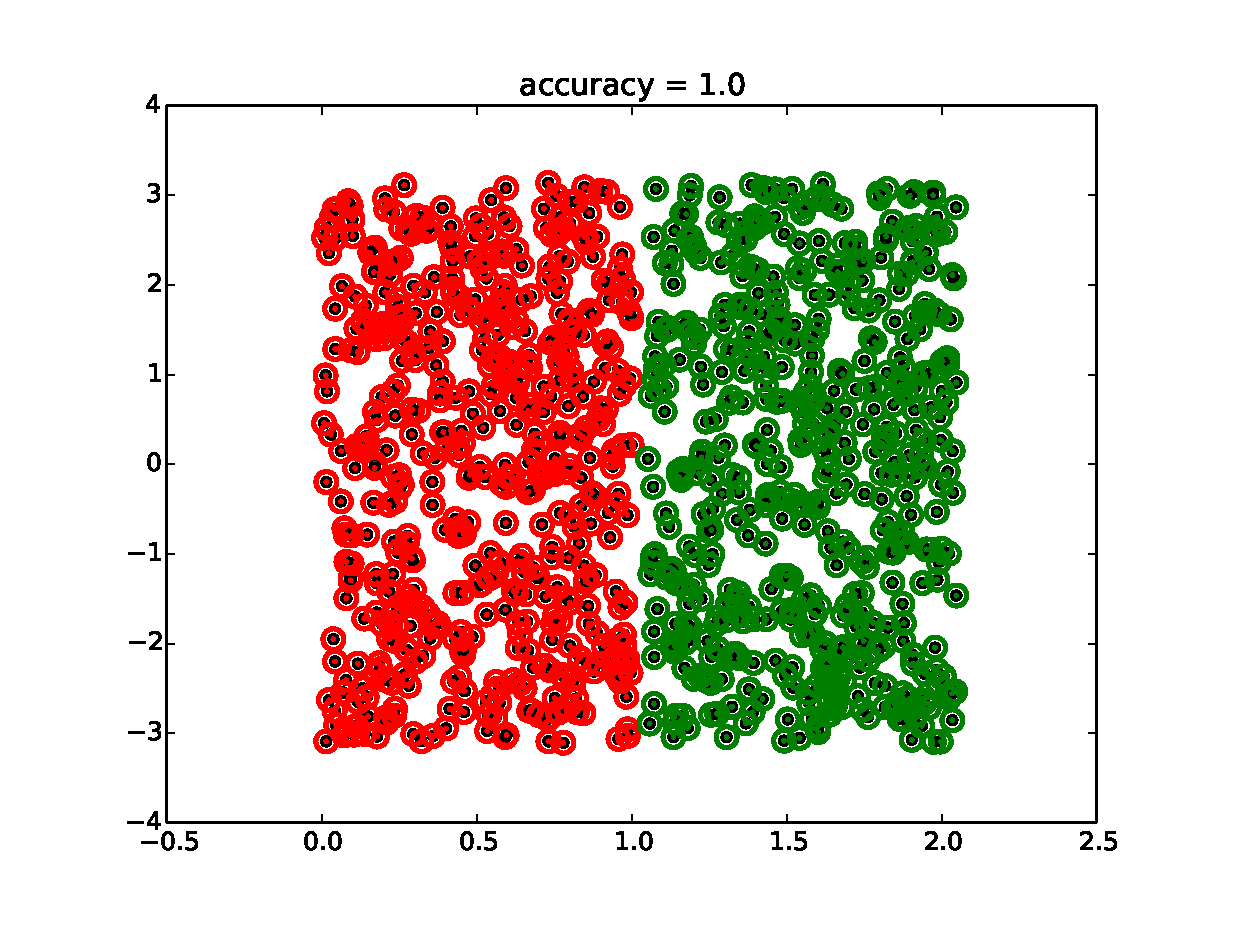
\includegraphics[width=0.49\textwidth]{linearSVMonPolar.eps}
    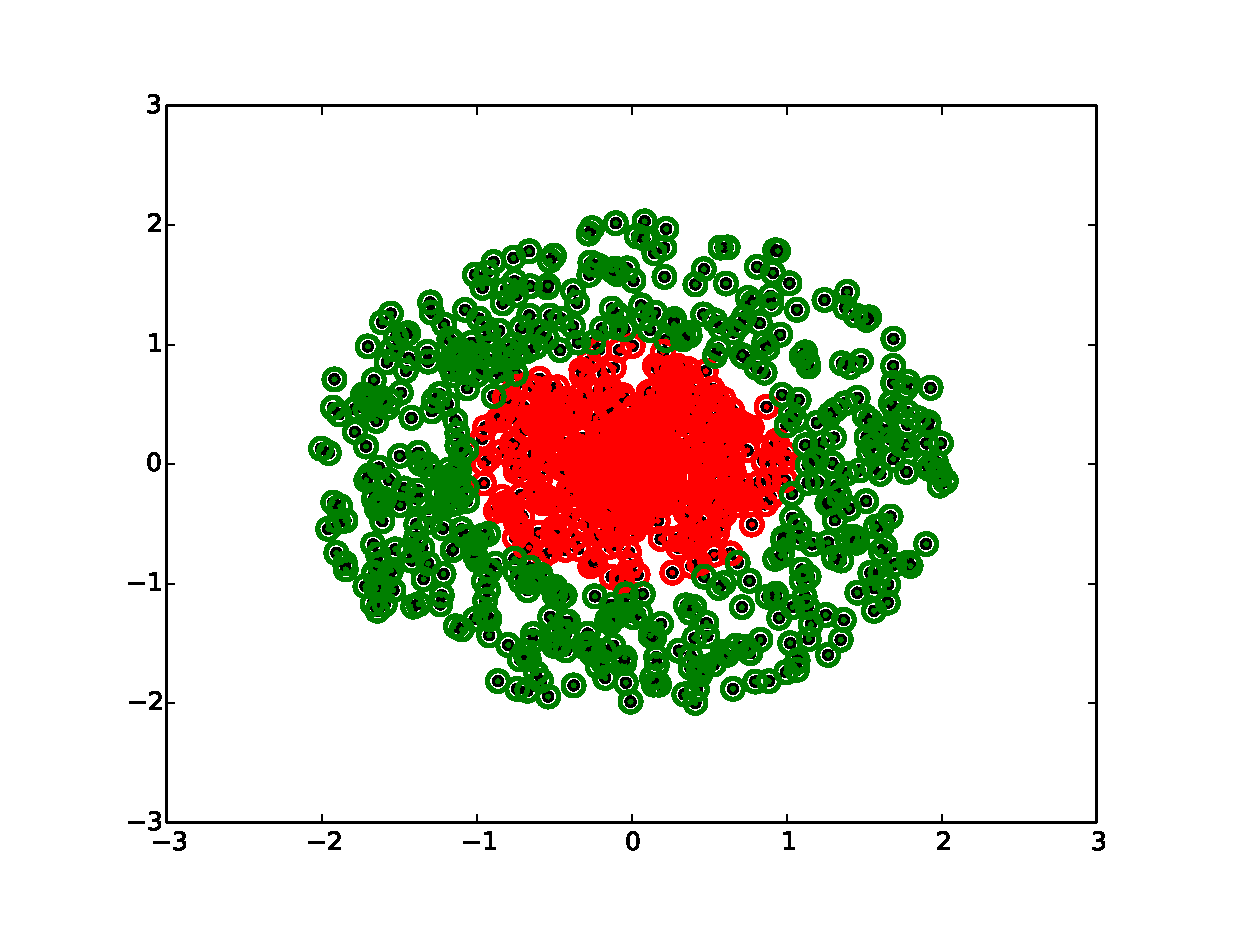
\includegraphics[width=0.49\textwidth]{final.eps}
    \caption{Predicted classes on polar data using a linear SVM classifier, plotted also at their original coordinates.}
    \label{fig:linearSVMonPolar}
\end{figure}

\section{Image classification -- linear SVM}

\section{Image classification -- discussing the results}

\section{Image classification -- comparison $k$-NN vs SVM}


%\bibliographystyle{plain}
%\bibliography{thereference}
\end{document}
